\captionsetup{
    singlelinecheck=false,
    justification=justified
    }
\begin{figure}[htbp]
\begin{subfigure}[t][][t]{0.48\textwidth}
    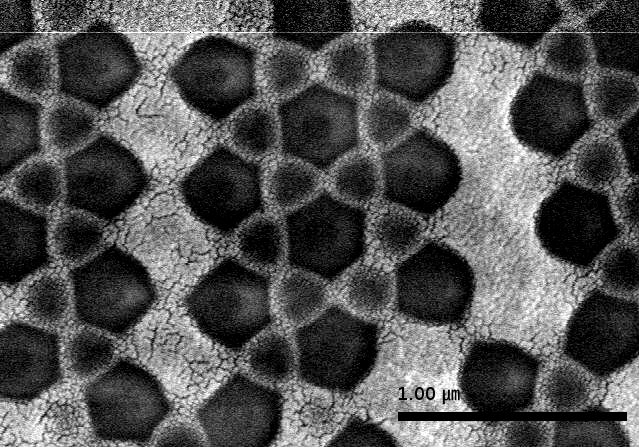
\includegraphics[width=\textwidth]{fr180-1_edited_bar.jpg}
    \caption[justification=raggedright]{
        Full-rings for \SI{180}{\second} annealing.\\
        One can clearly see the full-rings but they overlap.
        }
    \label{fig:sem-fr1}
\end{subfigure}
\hfill
\begin{subfigure}[t][][t]{0.48\textwidth}
    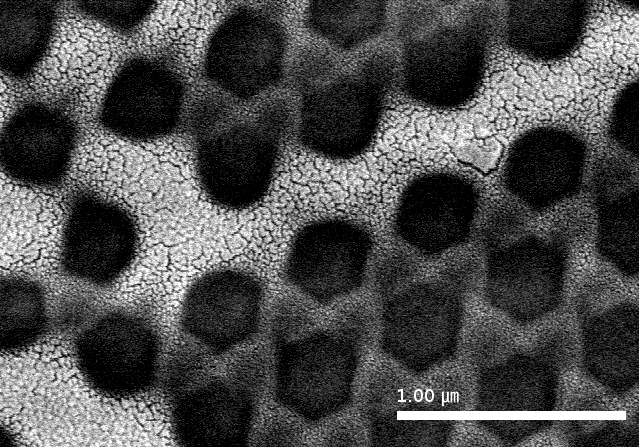
\includegraphics[width=\textwidth]{sr2180-2_edited3_bar.jpg}
    \caption{
        Split-rings for \SI{180}{\second} annealing.\\
        The split-rings are open at the lower left.
        They also overlap
    }
    \label{fig:sem-sr1}
\end{subfigure}

\begin{subfigure}[t][][t]{0.48\textwidth}
    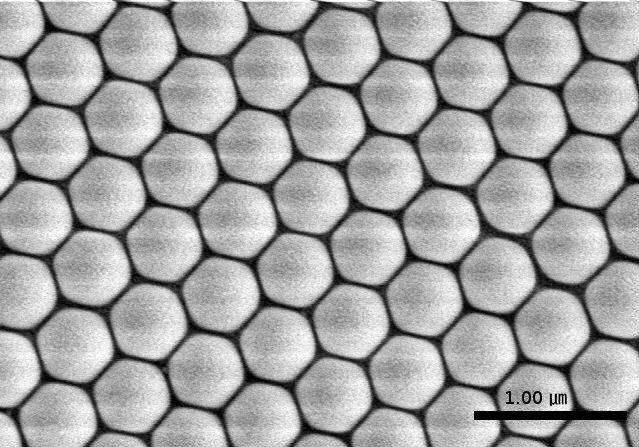
\includegraphics[width=\textwidth]{sr180-4_edited_bar.jpg}
    \caption{
        Mask for \SI{180}{\second} annealing.\\
        The image shows the hexagonal structure of the microspheres of the mask.
    }
    \label{fig:sem-mask}
\end{subfigure}
\hfill
\begin{subfigure}[t][][t]{0.48\textwidth}
    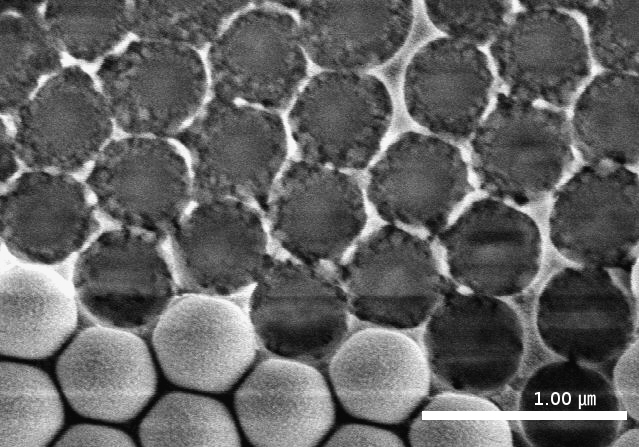
\includegraphics[width=\textwidth]{sr180-3_edited_bar2.jpg}
    \caption{
        Non sufficient annealing (\SI{180}{\second}).\\
        This image shows what happens when the probe was not annealed long enough.
        The gaps between the microspheres are not closed and gold is evaporated everywhere in between.
    }
    \label{fig:sem-nsa}
\end{subfigure}
\end{figure}
\begin{itemize}
    \item A scanning electron microscope uses a focused electron beam in a raster scan pattern.
    The following SEM images show the metamaterial probes.
    The bright areas are the gold films and the dark one are bare substrate.
    \item One can see that the produced rings overlap.
    This will disturb the expected metamaterial behavior because a current can flow from one ring to another.
    There are two possible explanations for this overlap:
    %A possible reasons for this overlap is insufficient annealing time.
    %The size of the holes in the mask is then too big.
    \begin{enumerate}
        \item Insufficient annealing time leads to too big holes in the mask.
        \item A too wide angle $\theta$ leads to too big ring diameters.
    \end{enumerate}
\end{itemize}



